\maketitle
\tableofcontents
\newpage

\section{Zielsetzung}
In diesem Versuch geht es um die Untersuchung der Wärmeleitung von Aluminium, Edelstahl und Messing
und die Bestimmung des Wärmeleitungskoeffizienten.
\section{Theorie}
Wärmeleitung ist eine von drei Methoden, um Wärme entlang eines Temperaturgefälles zu transportieren,
welches durch eine Störung des Temperaturgleichgewichts ensteht. Neben Konvektion und Wärmestrahlung
erfolgt die Wärmeleitung durch Phononen und frei bewegliche Elektronen. Durch einen Stab der Länge L und der
Querschnittsfläche A, der aus einem Material mit Dichte $\textit{\rho}$ und spezifische Wärme $\textit{c}$ besteht,
fließt in der Zeit d$\textit{t}$ bezüglich der Querschnittsfläche die Wärmemenge
\begin{equation}
  \symup dQ = - \kappa \, A \, \frac{\partial T}{\partial x} \, \symup dt .
  \label{eqn:1}
\end{equation}
Dabei ist $\kappa$ die materialabhängige Wärmeleitfähigkeit. Mit Hilfe der Wärmestromdichte
$j_{\omega}$ und Wärmeleitungsgleichung lässt sich die Temperaturwellengleichung schreiben als
\begin{equation}
  T(x, t) = T_{max} \ e^{\sqrt{\frac{\omega \rho c}{2 \kappa}} \, x} \,
  cos \left(\omega t - \sqrt{\frac{\omega \rho c}{2 \kappa}} \, x \right)
  \label{eqn:2}
\end{equation}
für einen mit Periode T abwechselnd erwärmten und abgekühlten sehr langen Stab.
Die Phasengesschwindigkeit der Welle lautet
\begin{equation}
    v = \frac{\omega}{k} = \frac{\omega}{\sqrt{\frac{\omega \rho c}{2 \kappa}}}
    = \sqrt{\frac{2 \kappa \omega}{\rho c}}
    \label{eqn:3}
\end{equation}
zur Bestimmung der Dämpfung nutzt man das Amplitudenverhältnis aus $A_{nah}$ und $A_{fern}$
an zwei Messstellen $x_{nah}$ und $x_{fern}$. Für die Wärmeleitfähigkeit erhält man also
\begin{equation}
  \kappa = \frac{\rho c (\symup \Delta x)^2}{2 \, \symup \Delta t \, ln (A_{nah}/{A_{fern})}}
  \label{eqn:4}
\end{equation}
mit $\symup \Delta x$ als Abstand und $\symup \Delta t$ als Phasendifferenz der Temperaturwelle
zwischen den beiden Messstellen.
\section{Durchführung}
\subsection{Versuchsaufbau}
Auf der Grundplatte sind vier rechteckige Probestäbe aus Aluminium, zweimal Messing
und Edelstahl. Ein Peltierelement erhitzt bzw. kühlt die Probestäbe gleichzeitig.
Mit einem Schalter lässt sich zwischen diesen beiden Betriebsarten umschalten, siehe \ref{fig:1}.
Die Eingangsspannungen sind \SI{5}{\volt} für die statische bzw. \SI{8}{\volt}
für die dynamische Methode \footnote{Siehe \ref{sec:1}}. Die Temperaturen werden
an zwei Stellen eines Stabes abgegriffen und an einen Datenlogger (Xplorer GLX)
weitergeleitet.
\begin{figure}[t]
  \centering
  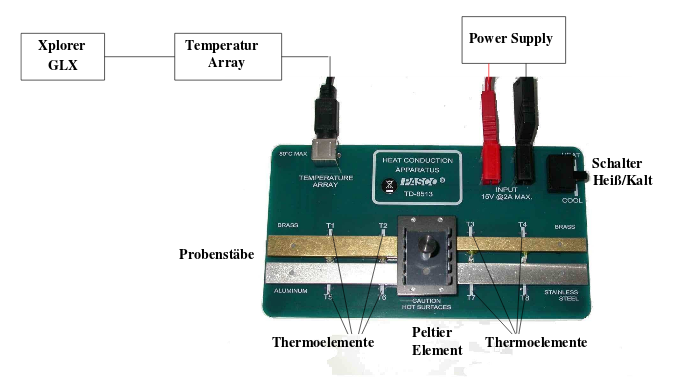
\includegraphics[scale=0.5]{versuchsaufbau.png}
  \caption{Grundplatte mit vier Probestäben, dem Peltier-Element und den nötigen Anschlüssen
  für Strom und Datenlogger.}
  \label{fig:1}
\end{figure}
\begin{figure}
  \centering
  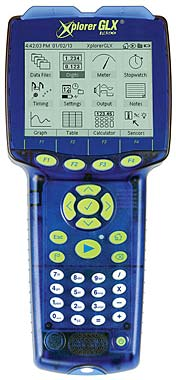
\includegraphics[scale=0.5]{xplorer_glx.jpg}
  \caption{Darstellung eines Datenloggers Typ Xplorer GLX.}
  \label{fig:2}
\end{figure}
\subsection{Versuchsdurchführung}
\label{sec:1}
Zu Beginn des Versuchs und nach jedem Abkühlvorgang isolieren wir die Metallstäbe,
um den Wärmeaustausch mit der Umgebungs so gering wie möglich zu halten. Es werden
zwei verschiedene Messmethoden angewandt:
\begin{itemize}
  \item $\textbf{Statische Methode:}$
    Über den zeitliche Temperaturverlauf wird die Wärmeleitfähigkeit bestimmt.
    Zu diesem Zweck werden an zwei Messstellen eines jeden Metallstabs die Temperatur
    als Funktion der Zeit dargestellt, was eine Gesamtanzahl von acht Sensoren bedeutet.
    Mit einer Abtastrate von \SI{5}{\second} und einer wie oben
    bereits erwähnten Spannung von \SI{5}{\volt} wird die erste Messung durchgeführt,
    bis der siebte Sensor ungefähr \SI{45}{\celsius} anzeigt. Nach Beendigung der Messunge
    werden die Probestäbe abgekühlt.

  \item $\textbf{Dynamische Methode:}$ Wir verwenden als dynamische Methode in diesem
    Versuch die Angström-Methode, die sich dadurch auszeichnet, dass der Stab periodisch erhitzt wird.
    In diesem Fall wir die Wärmeleitfähigkeit aus der Ausbreitungsgeschwindigkeit der
    Temperaturwelle berechnet. Die Abtatstrate bei dieser Methode beträgt \SI{2}{\second}
    und die Spannung \SI{8}{\volt}.
    Wenn die Thermoelemente eine Temperatur von \SI{30}{\celsius} oder niedriger erreicht haben,
    führt man die nächste Messung durch, indem man für eine Periode von \SI{80}{\second}
    eine Temperaturwelle erzeugt. Dies geschieht, wenn man nach \SI{40}{\second} heizen für
    wiederum \SI{40}{\second} mithilfe des Peltierelements die Probestäbe abkühlt.
    Nach zehn solcher Perioden ist die Messung beendet. Nachdem die Probestäbe wie bei der
    statischen Methode hinreichend abgekühlt sind, führt man noch eine Messung mit einer
    Periodendauer von \SI{200}{\second} für neun
    Perioden durch. Wenn eins der Thermoelemente \SI{80}{\celsius} anzeigt, wird die Messung gestoppt.
    Die Messtäbe werden anschließend wieder gekühlt.
\end{itemize}
\section{Fehlerrechnung}
Es gibt:
\begin{equation}
  \bar{T} = \frac{1}{n} \sum_{i=1}^{n} T^{i}
  \label{eqn:5}
\end{equation}
den Mittelwert und:
\begin{equation}
  \sigma_{\bar{T}} = \sqrt{\frac{1}{n(n-1)} \sum_{i=1}^{n}(\bar{T}-T_i)^2}
  \label{eqn:6}
\end{equation}
den Fehler des Mittelwertes.
\section{Auswertung}
\subsection{Statische Methode}
Alle Temperaturverläufe haben einen exponentiellen Verlauf.
Die Betrachtung der Temperaturverläufe an den entfernt liegenden Termoelementen zeigt, dass Aluminium die höchste
Wärmeleitfähigkeit besitzt. Auf Aluminium folgen Messing und schließlich Edelstahl, welches die geringste Wärmeleitfähigkeit der
betrachteten Metalle aufweist. Aus dem Verlauf der Temperaturkurven der beiden Messingstäbe folgt, dass aus einem höherer Querschnitt
eine höhere Wärmeleitung folgt.
\begin{figure}[h]
  \centering
  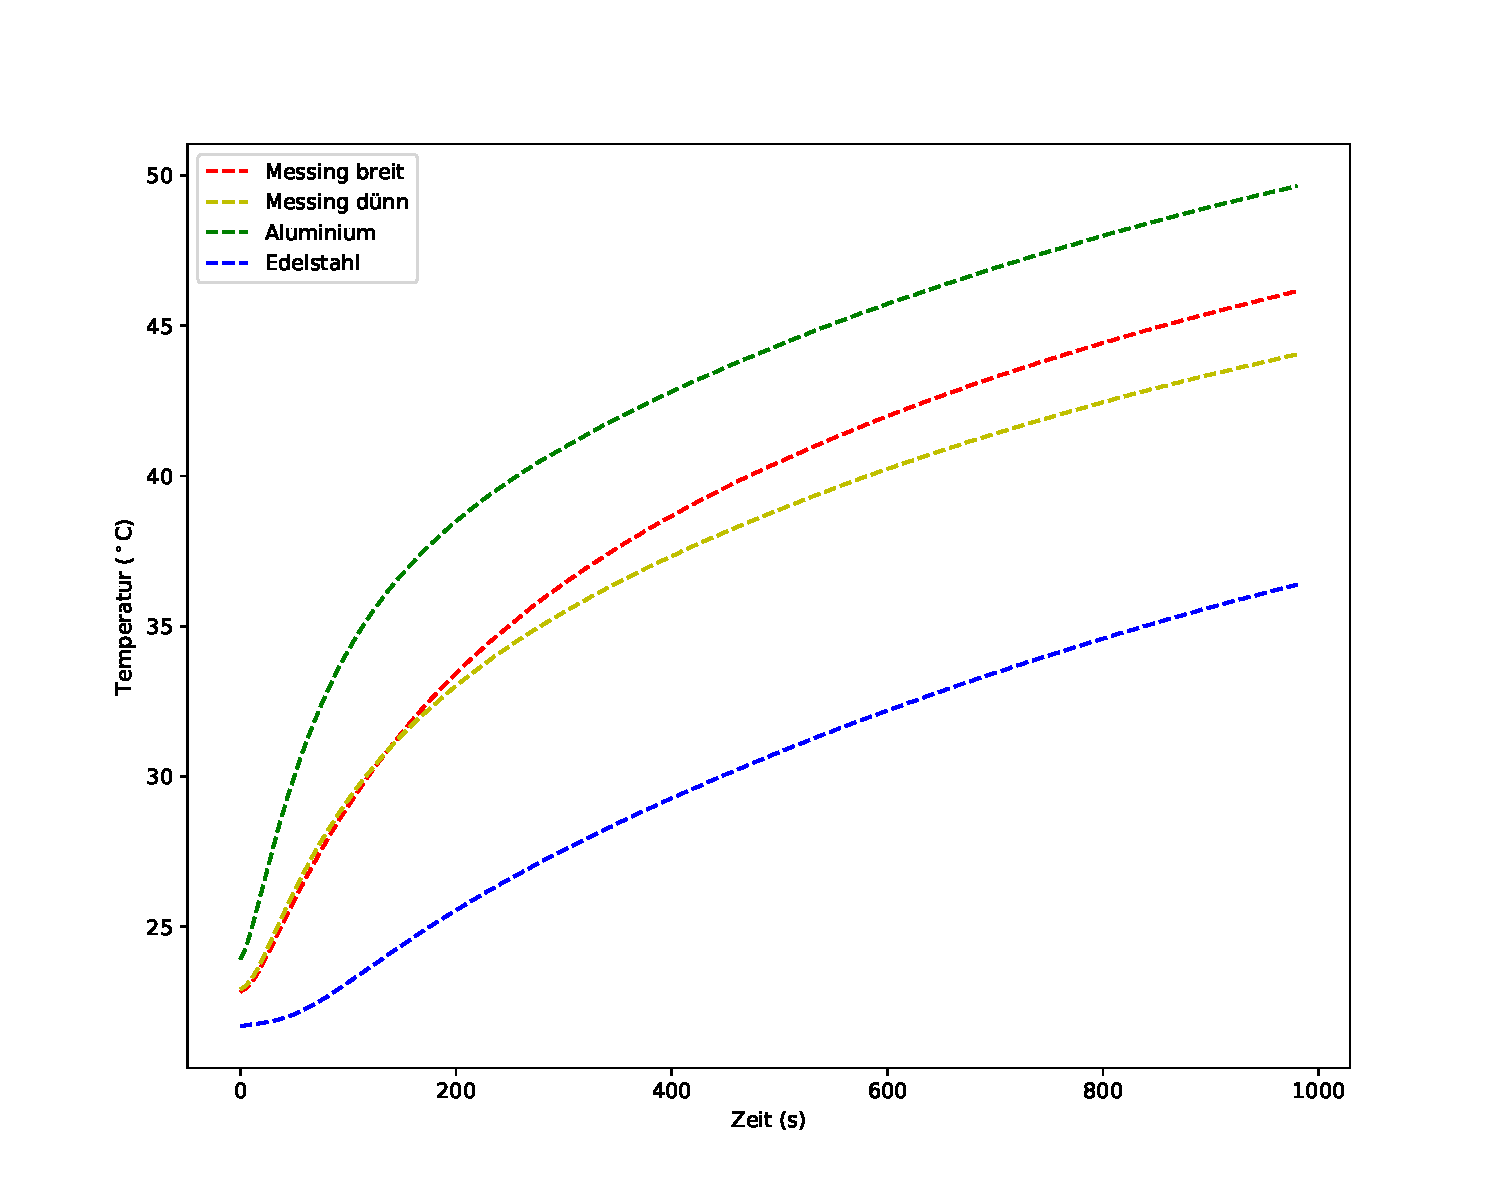
\includegraphics[scale=0.6]{Statisch.pdf}
  \caption{Temperaturverlauf der fernen Thermoelemente.}
  \label{fig:3}
\end{figure}
Bei der Temperaturdifferenz zeigen sich Unterschiede zwischen Messing und Edelstahl. Zuerst steigen beide Kurven stark an. Nach dem
Anstieg bleibt die Temperaturdifferenz des Edelstahls bis auf geringe Änderungen konstant. Beim Messing hingegen, fällt die Temperaturdifferenz
nach einem schnell erreichten Maximum exponentiell ab, bis es sich einem Konstanten Wert annähert. Dies zeigt sich auch im Wärmestrom nach \eqref{eqn:1} bei einem
Querschnitt von $A = \SI{4.8e-5}{\metre\square}$ über eine Länge von $\SI{0,03}{\metre}$:
\begin{table}[h]
  \centering
  \caption{Temperaturdiffernzen}
  \label{tab:deltaT}
  \begin{tabular}{S S S S S S}
    \toprule
    \multicolumn {3}{c}{Edelstahl, $\kappa = \SI{58}{\watt\per\metre\kelvin}$} & \multicolumn {3}{c}{Messing, $\kappa = \SI{120}{\watt\per\metre\kelvin}$} \\
    {$t$ in $\si{\second}$} & {$\symup \Delta T$ in $\si{\kelvin}$} & {$\symup \Delta Q / \symup \Delta t$ in $\si{\watt}$} & {$t$ in $\si{\second}$} &
      {$\symup \Delta T$ in $\si{\kelvin}$} & {$\symup \Delta Q / \symup \Delta t$ in $\si{\watt}$} \\
    \midrule
    100 & 281,00 & -26,08 & 50 & 277,28 & -53,24\\
    200 & 281,92 & -26,16 & 100 & 277,05 & -53,19\\
    400 & 281,88 & -26,16 & 150 & 276,62 & -53,11\\
    600 & 281,84 & -26,16 & 400 & 275,93 & -52,98\\
    800 & 281,77& -26,15 & 600 & 275,82 & -52,96\\
    \bottomrule
  \end{tabular}
\end{table}
Der Wärmestrom zeigt auch noch einmal, dass in Edelstahl bei der gleichen Erhitzung über die gleiche Distanz bei gleichem Querschnitt ein betragsmäßig
geringerer Wärmestrom fließt, Messing also besser Wärme leitet.

\subsection{Dynamische Methode}
Aus den Messungen folgen die in den Tabellen \ref{tab:Messing}, \ref{tab:Alu} und \ref{tab:Edelstahl} dargestellten Werte für die Amplituden sowie die Phasendifferenz.
Tabelle \ref{tab:MW} zeigt die Mittelwerte der Logarithmen der Amplitudenverhältnisse, sowie der Phasendifferenzen. Die Werte berechnen sich nach \eqref{eqn:5} für den
Mittelwert und \eqref{eqn:6} für den Fehler des Mittelwertes. Diese Werte geben nach \eqref{eqn:4} folgende Werte für $\kappa$:

\begin{table}[b]
  \centering
  \caption{Mittelwert der Logarithmen der Amplitudenverhältnisse sowie der Phasendifferenzen}
  \label{tab:MW}
  \begin{tabular}{c c c}
    \toprule
    Metall & $\overline{ln(\frac{A_{nah}}{A_{fern}})}$ & $\overline{\symup \Delta t} \text{ in } \si{\second}$\\
    \midrule
    Messing & 0.89 \pm 0.04 & 17.6 \pm 1.0 \\
    Aluminium & 0.62 \pm 0.04 & 10.2 \pm 0.6 \\
    Edelstahl & 1.64 \pm 0.11 & 59.7 \pm 1.6 \\
    \bottomrule
  \end{tabular}
\end{table}
\begin{equation*}
  \begin{split}
    \kappa_{Messing} = \SI{94(7)}{\watt\per{\metre\kelvin}} \\
    \kappa_{Aluminum} = \SI{166(14)}{\watt\per{\metre\kelvin}} \\
    \kappa_{Edelstahl} = \SI{14.7(10)}{\watt\per{\metre\kelvin}}
  \end{split}
\end{equation*}
\begin{table}[b]
  \centering
  \caption{Amplituden und Phasendifferenzen für Messing}
  \label{tab:Messing}
  \begin{tabular}{c c c c}
    \toprule
    $A_{nah} \text{ in } \si{\kelvin}$ & $A_{fern} \text{ in } \si{\kelvin}$ & $\symup \Delta t \text{ in } \si{\second}$ & $ln(\frac{A_{nah}}{A_{fern}})$\\
    \midrule
    13.64 & 7.48 & 21.75 & 0.60 \\
    12.32 & 5.72 & 21.75 & 0.77 \\
    11.88 & 5.28 & 21.75 & 0.81 \\
    11.44 & 4.84 & 17.40 & 0.86 \\
    11.00 & 4.40 & 17.40 & 0.92 \\
    11.00 & 4.40 & 17.40 & 0.92 \\
    11.00 & 4.40 & 17.40 & 0.92 \\
    10.56 & 3.96 & 15.22 & 0.98 \\
    10.12 & 3.52 & 13.05 & 1.06 \\
    10.12 & 3.52 & 13.05 & 1.06 \\
    \bottomrule
  \end{tabular}
\end{table}

\begin{table}[b]
  \centering
  \caption{Amplituden und Phasendifferenzen für Aluminium}
  \label{tab:Alu}
  \begin{tabular}{c c c c}
    \toprule
    $A_{nah} \text{ in } \si{\kelvin}$ & $A_{fern} \text{ in } \si{\kelvin}$ & $\symup \Delta t \text{ in } \si{\second}$ & $ ln(\frac{A_{nah}}{A_{fern}}) $ \\
    \midrule
    19.24 & 13.32 & 11.10 & 0.37 \\
    16.65 & 10.36 & 8.88 & 0.47 \\
    15.91 & 8.88 & 8.88 & 0.58 \\
    15.54 & 8.14 & 11.10 & 0.65 \\
    14.80 & 7.77 & 6.66 & 0.64 \\
    14.80 & 7.77 & 13.32 & 0.64 \\
    14.43 & 7.40 & 8.88 & 0.67 \\
    14.43 & 7.03 & 11.10 & 0.72 \\
    14.43 & 7.03 & 11.10 & 0.72 \\
    14.06 & 7.03 & 11.10 & 0.69 \\
    \bottomrule
  \end{tabular}
\end{table}

\begin{table}[b]
  \centering
  \caption{Amplituden und Phasendifferenzen für Edelstahl}
  \label{tab:Edelstahl}
  \begin{tabular}{c c c c}
    \toprule
    $A_{nah} \text{ in } \si{\kelvin}$ & $A_{fern} \text{ in } \si{\kelvin}$ & $\symup \Delta t \text{ in } \si{\second}$ & $ln(\frac{A_{nah}}{A_{fern}})$\\
    \midrule
    5.50 & 1.65 & 54.60 & 1.20 \\
    3.52 & 0.77 & 59.15 & 1.52 \\
    1.98 & 0.22 & 54.60 & 2.20 \\
    3.85 & 0.77 & 63.70 & 1.61 \\
    3.52 & 0.77 & 63.70 & 1.52 \\
    3.41 & 0.55 & 63.70 & 1.82 \\
    4.07 & 0.66 & 54.60 & 1.82 \\
    4.51 & 1.10 & 63.70 & 1.41 \\
    \bottomrule
  \end{tabular}
\end{table}

Im Vergleich mit Literaturwerten \cite{literaturwerte}:
\begin{equation*}
  \begin{split}
    \kappa_{Messing} = \num{81}\text{... }\num{105}\,\si{\watt\per{\metre\kelvin}} \\
    \kappa_{Aluminum} = \SI{220}{\watt\per{\metre\kelvin}} \\
    \kappa_{Edelstahl} = \SI{15}{\watt\per{\metre\kelvin}}
  \end{split}
\end{equation*}
zeigt sich, dass die aus der Messung für Messing und Edelstahl folgenden Werte im Bereich der Messtoleranz liegen.
Für Aluminium ist dies nicht der Fall.

\section{Diskussion}
Zusammenfassend zeigen sich gute Ergebnisse, die großteils mit der Literatur übereinstimmen. Lediglich bei Aluminium ist die Abweichung groß. Fraglich ist an dieser Stelle, welche Legierung für Messing und Edelstahl verwendet wurden, sowie wie rein das Aluminium ist. Es kann somit
keine absolut verlässliche Aussage getroffen werden, inwieweit die für die Metalle gefundenen Literaturwerte mit den verwendeten Materialien übereinstimmen. Insbesondere bei Messing
wir in der Literatur ein Intervall angegeben, in dem sich auch der aus der Messung folgende Wert findet.
Mögliche systematische Fehlerquellen können hier die Abschirmung der Stäbe sein. Da diese nicht perfekt ist, findet trotzdem
ein Wärmeaustausch mit der Umgebung statt. Statistische Fehler können sich durch die Auswertungsmethode ergeben. Hier mussten
mit Lineal die Amplituden und Phasendifferenzen aus Grafiken abgelesen werden. Die dabei zwangsläufig entstehenden Ablesefehler lassen sich
nicht quantifizieren und finden sich am Ende trotz Bildung des Mittelwertes im Ergebnis wieder.
\\
\\
Generell lassen sich durch die digitale Datenerfassung aber viele Fehlerquellen ausschließen. Eine weitere Steigerung der Messgenauigkeit könnte
durch eine komplett digitale Auswertung erreicht werden, wodurch die Ablesung mit Lineal wegfallen würde. Eine weitere Steigerung der Abschirmungsgüte
lässt sich bei der geringen Größe der Petier-Elemente nur schwer erreichen. Hier könnten bessere Dämmaterialien eingesetzt werden.

\newpage
\nocite{*}
\printbibliography
